% The diagram on Figure \ref{fig:processing_flow} illustrates the proposed methodology to achieve the extended depth of field. The framework can be divided into four parts, as follows:

% \begin{figure}[H]
% 	\centering
% 	\caption{\label{fig:processing_flow}Generic processing flow of the extended depth of field task: Image Acquisition \textbf{(I)}, Image Pre-processing \textbf{(II)}, Image Segmentation \textbf{(III)}, Image Fusion \textbf{(IV)} and Evaluation \textbf{(V)}.}
% 	\begin{center}
% 	    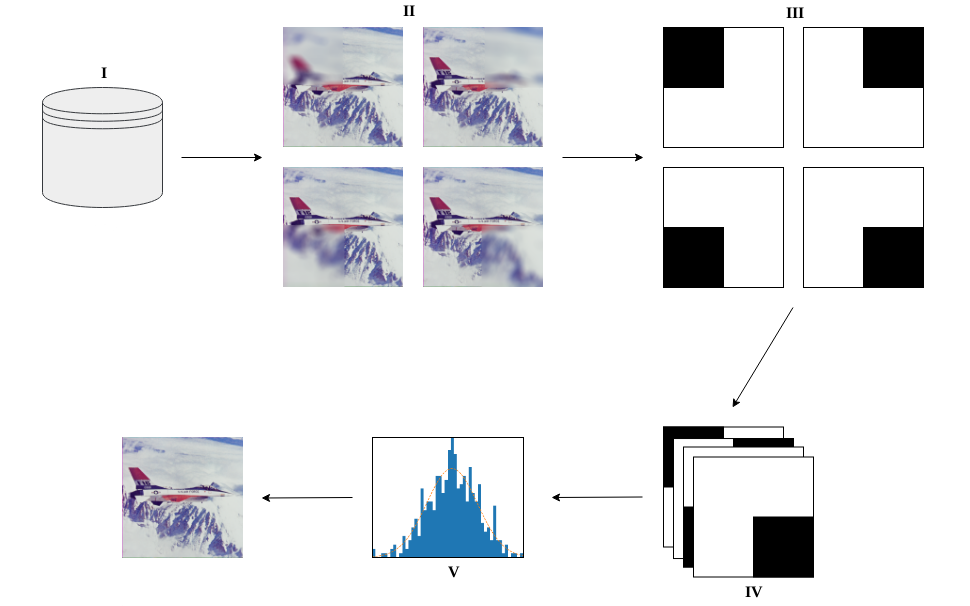
\includegraphics[scale=0.35, trim = {0 0.3cm 0 2cm}]{images/fig12.png}
% 	\end{center}
% 	\centering
%     \fautor
% \end{figure}

% \begin{enumerate}[label=\Roman*.]
%     \item \textbf{Image Acquisition}: several images will be acquired in different focus settings with the light microscope. The AxioVision 4.8 acquisition module tool called \emph{Z-Stack} allows to acquire images along the $z$ axis with a motorized focusing device that provides steps between each image with micrometer scale precision. This will result in a set of images with different levels of blur;
    
%     \item \textbf{Image Pre-processing}: some adjustments are necessary prior to segmentation. The original image stack is in the RGB colour space. There was a conversion to colour spaces such as the \sigla{HSV}{Hue, Saturation and Value colour space}, in which the Value channel may be used for processing, the \sigla{LAB}{Lightness and colour-opponent dimensions A and B} where the Lightness channel could be processed or just a conversion from RGB to grayscale in order to perform tests. This process is reversible, so that images can be presented in their original RGB colour space;
    
%     \item \textbf{Image Segmentation}: images will go through a process of splitting the pixels in blurred and sharp groups. This step will locally scan the pixels in some transform domain (\textit{a priori}, in the Fourier domain) in order to label them in one of the groups. In a nutshell, this will either produce a matrix of zeros and ones with the same dimensions of the image, or a set of regions labeled as blurry or sharp (which depends on the chosen window size for STFT, for example). This represents the blur maps and will work as input to carry out the fusion step;
    
%     \item \textbf{Image Fusion}: the step consists of scanning the blur maps and selecting the sharp regions in each image; these will be merged so as to minimize overlaps, and the final result will be a mostly or fully sharp image. The blur maps contain information about each sharp region of each image, and the image fusion process will choose the sharpest pixels to compose the resulting image based on the blur map and a numerical metric; the former may be based on pixel-level or transform domain level approaches.
    
%     \item \textbf{Evaluation}:  evaluate the quality of the segmentation procedure and also compare the sharpness level of the fused image with other images. This will allow to gauge the reliability of the processes and determine whether a) the process should be repeated; b) the parameters of the algorithms are well estimated and c) the algorithm itself is performing well. The final image fusion result will be evaluated with error-based methods and the segmentation quality will have probability measurements of precision, in comparison to the ground truth images. 
% \end{enumerate}

% The next sections will provide details on the data to be processed and relevant information on the techniques that will be used to fulfill the proposal.

% \section{Materials}

% To precisely validate the segmentation process, a set of \emph{ground truth} images with structures of well-known dimensions, formats and known blurry regions is required. This can be done by imaging a set of objects such as coins, crystals and stones. It is also possible to blur sharp structures by the convolution of a known blur kernel with a sharp image. 

% This can be directly applied in order to obtain higher quality in plant leaf histological samples, which have a specific structured called \emph{stoma}, responsible for gas exchanges with the surrounding medium. \emph{Stomata} exhibit a non-regular topology which leads to defocus blur while acquiring images. There are several works on plant leaf images done by the  \sigla{SCG}{Scientific Computing Group} in \sigla{IFSC}{São Carlos Institute of Physics}, including biological studies with complex network analysis, as the stomata were modelled as graphs. Figure \ref{fig:validation_images} shows how the test images may look like:

% \begin{figure}[htb]
% 	\centering
% 	\caption{\label{fig:validation_images}Images that may be used for evaluating the algorithm: (a) partially blurred airplane with an artificial gaussian blur kernel, (b) a 300x magnified contact pad for the electrical interface on the front side of a credit card , (c) surface of a 300x magnified Brazilian 5 \emph{centavos} coin and (d) 50x magnified \textit{Callisia repens} specimen, where it is possible to see stomata and a blurry background.}
% 	\begin{center}
% 	    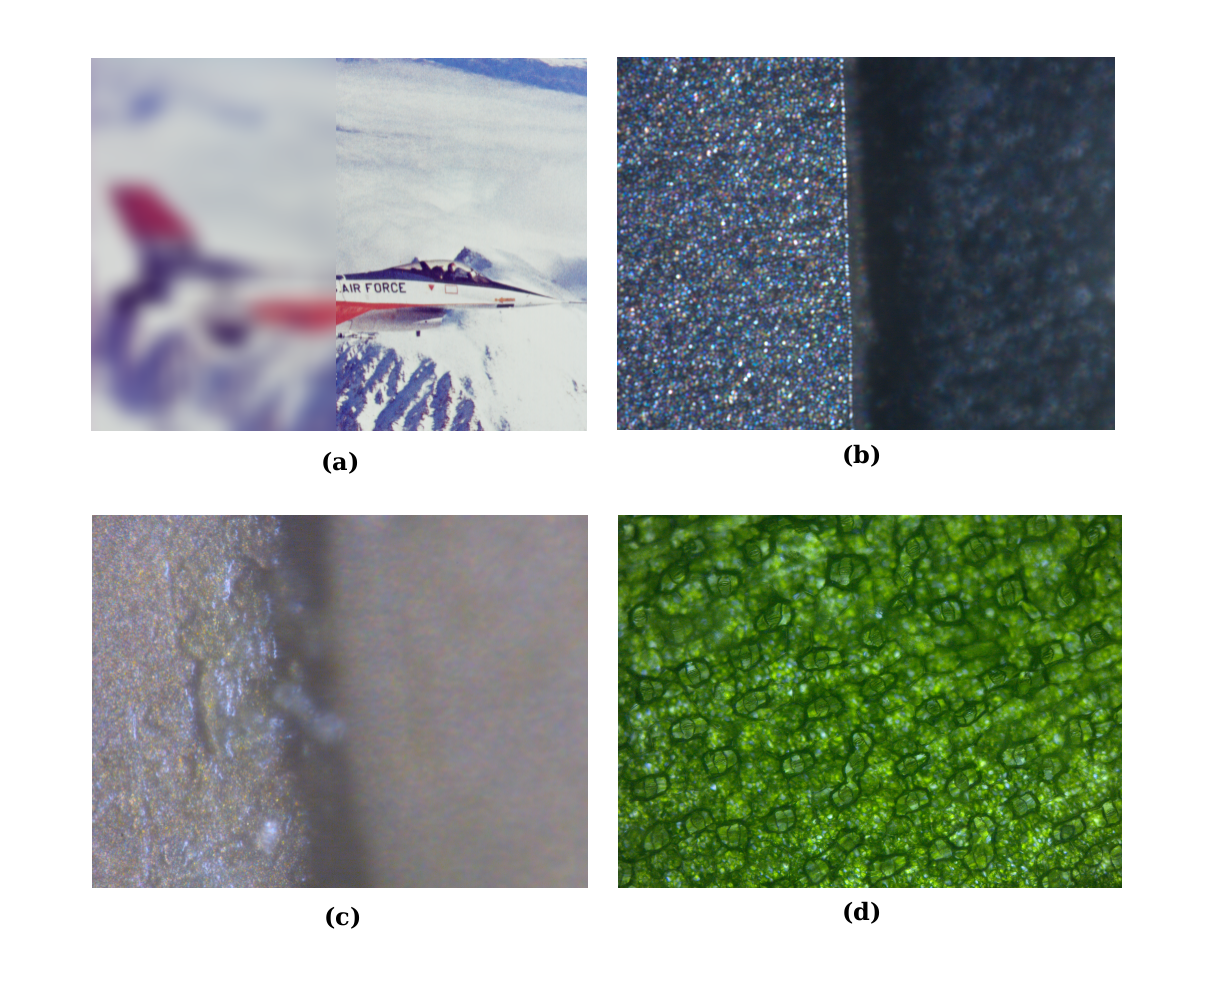
\includegraphics[scale=0.35]{images/fig13.png}
% 	\end{center}
% 	\centering
%     \fautor
% \end{figure}

% The images will be acquired with a ZEISS SteREO Discovery.v20 stereo compound microscope. This microscope is used for three-dimensional observations of small objects, with applications in biology, medicine and tissue examination \cite{stereo2012carl}. Figure \ref{fig:stereo_v20} illustrates a stereo compound light microscope from the SCG group that was used to obtain images \ref{fig:validation_images}.\textbf{(b)}, \ref{fig:validation_images}.\textbf{(c) }and \ref{fig:validation_images}.\textbf{(d)}.

% \begin{figure}[H]
% 	\centering
% 	\caption{\label{fig:stereo_v20}Zeiss SteREO v20 microscope from the SCG group.}
% 	\begin{center}
% 	    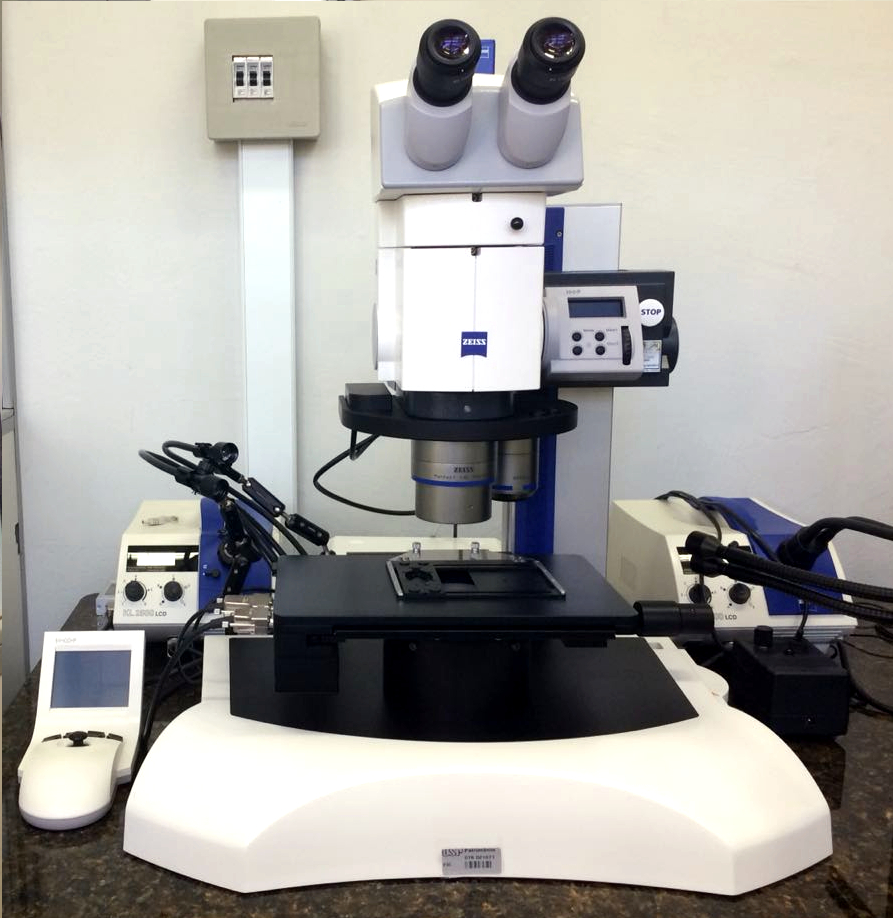
\includegraphics[scale=0.3]{images/fig14.png}
% 	\end{center}
% 	\centering
%     \fautor
% \end{figure}

\section{Methods}

\subsection{Discrete Fourier Transform based no-reference image quality assessment}
teste

\subsection{Energy of Laplacian based Image Fusion}
teste 2


% One of the pre-processing tasks consists of colour space conversion, from RGB to HSV and LAB , or to grayscale for testing purposes only. A noise reduction procedure may also be necessary, since microscopy images have a considerable amount of noise. If the amount of noise is created by the texture of the surface, e.g. the coin surface, which shows a particle pattern when magnified, noise reduction procedures should not be done as pre-processing.

% According to the literature review from chapter \ref{chapter:related-work}, both segmentation and fusion procedures depend on the problem and should have their parameters optimized empirically. There are several approaches applied by image segmentation algorithms such as pixel-level analysis, region based segmentation, edge based segmentation and so on. Those which are done in the spatial domain have a high computational cost and also a high computational complexity, and are designed for tasks where the segmentation appears to be simple. For region-based segmentation, there are techniques that rely on other mathematical frameworks, e.g. transform domain methods, statistical analysis and linear algebra, as shown in chapter \ref{chapter:related-work}. This work proposes a region-based image segmentation method within transform domains.

% The first proposed method for blur segmentation lies upon FFT analysis to identify images with low degree of blur. The most trivial method to be tested is the computation of spectral energy density in frequency bands of the global FFT. The energy in this contexts is somehow related to its concept is physics: the amount of some quantity that should be transferred to something in order to promote the increase or decrease of some property, e.g. the transfer of heat in order to increase the temperature. In this case, spectral energy density consists of the frequency response of the amount of photons which were transferred to the sensor when the image was acquired. The energy can be computed with the $L_{2}$ norm as described in equation \ref{eqn:spectral_energy_density}:

% \begin{equation}
% \label{eqn:spectral_energy_density}  
%     E = \sum_{x=0}^{M-1}\sum_{y=0}^{N-1}|F(x,y)|^{2}
% \end{equation}

% \noindent where $F$ is the FFT coefficients from the transformed image, $M$ and $N$ are the dimensions of the spectrum. The frequency bands, considering the shift of smallest coefficients to the center of the spectrum, the center as an origin for a coordinate system and the image dimensions as $N$x$N$, consists of lower frequencies in circles around the center (with radius $r < N/2$), medium frequencies when $r$ is close to $N/2$ and high frequencies when $r > N/2$. The idea is that blurry images have spectral energy density values with lower magnitudes, since the blurring process promotes a loss of details and is similar to low-pass filtering operation.

% The acquisition of the different bands in two-dimensional spectra can be made with circles centered at the zero frequency, shifted to the image central coordinate. Alternatively, the use of rectangles (or frames) may have similar effects due to the fact that the spectrum can be taken as a mixture of two one-dimensional spectra in each axis. In the end of the process,  images can be taken as sharp or blurry, considering the magnitude of the energy values.

% Following this approach, the next trial is to apply the two-dimensional STFT and also compute the energy in different bands. It is known that microscopy images suffer partial blur due to the depth of field feature. Therefore, local analysis may be used to obtain a precise blur map. The algorithm for computing the transform consists of the following steps:

% \begin{enumerate}[label=\Roman*.]
%     \item Generate a discrete two-dimensional window from two one-dimensional windows. The lengths of each window are taken as input, but it is mandatory that their dimensions originate a window that fits into the image;
    
%     \item Separate the image in slices of the same dimensions of the window. For each slice, perform the inner product between the image and the window;
    
%     \item For each windowed slice, perform the FFT.
% \end{enumerate}

% The result is a set of local FFTs. For blurred slices, higher energy values within the low--mid bands will be expected. 

% The next step is the image fusion. According to \citeonline{garg2014survey}, the spatial domain-based algorithms cause blur and are sensitive to noise, but contain reasonable information about positions of objects in the scene. Transform domain-based solutions are more complex to implement and also have a higher computational complexity in comparison its counterpart. Therefore, transform domain techniques alone, or a combination of both,  is suitable for this work.

% The proposed image fusion algorithm is based on the Fourier domain. Since the proposed segmentation procedure provides a blur map and transforms the image from the spatial domain to the Fourier domain, it is possible to use the information of the blur maps and also the remaining coefficients from the transform in order to perform image fusion. Considering that each coefficient represents a pixel in the original image, the image slices from the STFT on each of the multifocus images can be considered as a \emph{tensor} (a higher dimension array in this case). Figure \ref{fig:tensor} denotes a simple example of the tensor concept:

% \begin{figure}[H]
% 	\centering
% 	\caption{\label{fig:tensor}Graphical idea of a $8$x$8$x$8$ tensor, which arbitrarily represents the structure of the blur maps and the resulting Fourier spectra from the segmentation procedure.}
% 	\begin{center}
% 	    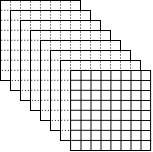
\includegraphics[scale=0.8]{images/fig15.png}
% 	\end{center}
% 	\centering
%     \fautor
% \end{figure}

% \noindent For each pixel of the image, which corresponds to one complex coefficient in one of the Fourier spectra, the average of the values should be calculated and the coefficient with the highest similarity will be chosen as the corresponding pixel to compose the fused image. If a set of coefficients has the same similarity when compared to the average value, it means that all related pixels have the same degree of sharpness, then the coefficient may be randomly chosen. 




% \section{Evaluation Methods}

% According to \citeonline{bovik2009mean}, the \sigla{MSE}{Mean Squared Error} is a measure of signal fidelity. Two signals are compared and a quantitative measure that describes the degree of similarity (fidelity), or the degree of error between them is computed. One indicator is considered as ideal and the other as a result of processes that may have distortions and inconsistencies. Considering $f (x, y)$ and $g (x, y)$ as two functions, the MSE can be represented by the equation \ref{eqn:mse}, and in a general way by equation \ref{eqn:mse_lp_norm}:

% \begin{equation}
% \label{eqn:mse}
% 	MSE =  \frac{1}{MN}\sum_{i=1}^{M}\sum_{j=1}^{N}(f(x,y) - g(x,y))^2
% \end{equation}

% \begin{equation}
% \label{eqn:lp_norm2}
% 	d_p(f,g) = \Bigg(\sum_{i=1}^{M}\sum_{j=1}^{N}|f(x,y) - g(x,y)|^{p}\Bigg)^{1/p}
% \end{equation}

% \begin{equation}
% \label{eqn:mse_lp_norm}
% 	MSE =  \frac{1}{MN}d_p(f,g)
% \end{equation}

% \noindent where $M$ and $N$ are the dimensions of both signals and $p$ is the $l_{p}$ norm value, defined as distance function $d:S$ x $S \rightarrow \mathbb{R}^2$. An important derivation of this measure is the RMSE, which is just the root square of the MSE value and changes the range of the metric. For image processing, the MSE is converted into the PSNR metric, which is defined by the equation \ref{eqn:psnr}:

% \begin{equation}
% \label{eqn:psnr}
% 	PSNR = 10\log_{10}\Bigg(\frac{L^2}{\sqrt{MSE}}\Bigg)
% \end{equation}

% \noindent where $L$ is the intensity range for each pixel, usually $[0,255]$.

% The resulting blur map from the segmentation process is an array with binary values; it is possible to quantitatively determine the reliability of the segmentation. According to \citeonline{choi2009survey}, the binary feature vector is one of the most common pattern representations, and the similarity and distance measures performed in these sets of information are important for grouping, sorting and analysing data.

% Two common similarity metrics, the Jaccard and Dice indices, are appropriate in this scenario. Both are comprised within the $[0,1]$ interval, where 1 is the complete similarity and 0 the complete discrepancy. Table \ref{tab:jaccard_contingency} represents the relationship between the presence and absence of the pixels in two sets A (ground truth segmentation) and B (segmented image).

%         \begin{table}[!hbt]
% 		% Center the table
% 		\begin{center}
% 		% Title of the table
% 		\caption{Contingency table for Jaccard and Dice similarity indices.}
% 		\label{tab:jaccard_contingency}
% 		% Table itself: here we have two columns which are centered and have lines to the left, right and in the middle: |c|c|
% 		\begin{tabular}{|c|c|c|c|}
% 			% To create a horizontal line, type 
%             \hline
%              & Presence (A) & Absence (A) & $\mathit{\sum}$\\
%     		\hline
%           	 Presence (B) & a & b & a + b\\
%     		\hline
%           	 Absence (B) & c & d & c + d\\
% 			\hline
%              $\mathit{\sum}$ & a + c & b + d & a + b + c + d\\
%             \hline
% 		\end{tabular}
% 		\end{center}
% 		\fautor
%       \end{table}
      
% In this work, $a$ is the number of pixels classified as blurred in both sets, $b$ is the number of pixels classified as blurred in B but not in A, $c$ is the number of pixels classified as blurred in A but not in B, and $d$ is the number of pixels classified as sharp in both sets. As a result, the Jaccard and Dice similarity indices can be described by the equations \ref{eqn:jaccard} and \ref{eqn:dice}, respectively:

% \begin{equation}
% \label{eqn:jaccard}
% 	S_{jaccard} = \frac{a}{a + b + c}
% \end{equation}

% \begin{equation}
% \label{eqn:dice}
% 	S_{dice} = \frac{2a}{2a + b + c}
% \end{equation}